\documentclass[../probability-notes.tex]{subfiles}
\begin{document}
    %%%%%%%%%%%%%%%%%%%%%%%%%%%%%%%%%%%%%%%%%%%%%%%%%%%%%%%%%%%%%%%%%%%%%%%%%%%
    \section{Parameter Estimation}
    In probability theory, we usually have the distribution known to us and we try to use this information to obtain theoretical results applicable on population of this distribution. However, in statistics, we are given the samples drawn from the population, and we are interested in estimating the parameters of this population. For instance, it can be known that the samples are drawn from a normal distribution and the objective is to use the samples to obtain the mean and variance of the normal distribution. It is possible to partially know the parameters in some cases, for example mean is unknown but the variance is known. Following are some methods to obtain the \emph{estimates} of these parameters.

    
    %%%%%%%%%%%%%%%%%%%%%%%%%%%%%%%%%%%%%%%%%%%%%%%%%%%%%%%%%%%%%%%%%%%%%%%%%%%
    \subsection{Maximum Likelihood Estimator}
    Maximum Likelihood Estimator or MLE is based on the idea to \textbf{find that value of $\theta$ that maximizes the probability of observing the given set of samples of the population}. Alternately, let $x_{i}$ for $i=1,2,\ldots,n$ be $n$ samples drawn from a population whose distribution is parametrized by $\theta$ (can be a vector as well). Then we define the likelihood function as
    \begin{align*}
        \text{likelihood\;} = f(x_{1}, x_{2}, \ldots, x_{n}|\theta)
    \end{align*}
    i.e., the joint probability (or density) of occurrence of all the samples under the given distribution for some value of $\theta$. We aim to maximize this likelihood to get the estimate of $\theta$. It is often the case that taking logarithm of both sides allows for an easy way of estimation. Note that both likelihood an log likelihood are maximized by the same value of estimator.\newline

    %%%%%%%%%%%%%%%%%%%%%%%%%%%%%%%%%%%%%%%%%%%%%%%%%%%%%%%%%%%%%%%%%%%%%%%%%%%
    \subsubsection{MLE for Bernoulli Variable}
    Suppose we observe $n$ independent samples from a Bernoulli process and the aim is to find the MLE for the probability of success.\newline
    Let $p$ denote the probability of success. Then,
    \begin{align*}
        P(X_{i} = x) &= p^{x}(1-p)^{1-x} \text{\; where $x$ is $0$ or $1$}\\
        \text{or, \;} P(X_{i} = x_{i}) &= p^{x_{i}}(1-p)^{1-x_{i}}
    \end{align*}
    Since all the samples are independent, the joint probability or likelihood is simply the product of all the probabilities
    \begin{align*}
        f(x_{1}, x_{2}, \ldots, x_{n}|p) &= p^{x_{1}}(1-p)^{1-x_{1}} \ldots p^{x_{n}}(1-p)^{1-x_{n}}\\
        &= p^{\sum_{i=1}^{x_{i}}} (1-p)^{n-\sum_{i=1}^{x_{i}}}\\
        log(f(x_{1}, x_{2}, \ldots, x_{n}|p)) &= {\sum_{i=1}^{x_{i}}}log(p) + (n-{\sum_{i=1}^{x_{i}}})log(1-p)
    \end{align*}
    Taking the derivative with respect to $p$ to maximize,
    \begin{align*}
        \frac{d}{dp}log(f(x_{1}, x_{2}, \ldots, x_{n}|p)) &= {\sum_{i=1}^{x_{i}}}\frac{1}{p} - (n-{\sum_{i=1}^{x_{i}}})\frac{1}{1-p} = 0\\
        \text{or,\;} \Aboxed{\hat{p} &= \frac{\sum_{i=1}^{n}x_{i}}{n}}
    \end{align*}
    which is the proportion of successful trials in the sample.


    %%%%%%%%%%%%%%%%%%%%%%%%%%%%%%%%%%%%%%%%%%%%%%%%%%%%%%%%%%%%%%%%%%%%%%%%%%%
    \subsubsection{MLE for Poisson Variable}
    Suppose that we observe $n$ random samples obtained from a poisson process. Recall
    \begin{align*}
        P(X = k) = \frac{e^{-\lambda} \lambda^{k}}{k!}
    \end{align*}
    Hence, the joint distribution can be written as
    \begin{align*}
        f(x_{1}, x_{2}, \ldots, x_{n}|p) &= \prod_{i=1}^{n} \frac{e^{-\lambda} \lambda^{x_{i}}}{x_{i}!}\\
        f(x_{1}, x_{2}, \ldots, x_{n}|p) &= \frac{e^{-n\lambda} \lambda^{\sum_{i=1}^{n} x_{i}}}{\prod_{i=1}^{n} x_{i}!}\\
        log(f(x_{1}, x_{2}, \ldots, x_{n}|p)) &= -n\lambda + (\sum_{i=1}^{n} x_{i})log(\lambda) - \sum_{i=1}^{n} log(x_{i}!)\\
        \frac{d}{dp}(f(x_{1}, x_{2}, \ldots, x_{n}|p)) &= -n + (\sum_{i=1}^{n} x_{i})\frac{1}{\lambda}\\
        &= 0\\
        \text{or, \;} \Aboxed{\hat{\lambda} &= \frac{\sum_{i=1}^{n} x_{i}}{n}}
    \end{align*}
    i.e., the average rate is simply the average of all the observed arrivals.

    
    %%%%%%%%%%%%%%%%%%%%%%%%%%%%%%%%%%%%%%%%%%%%%%%%%%%%%%%%%%%%%%%%%%%%%%%%%%%
    \subsubsection{MLE for Normal Variable}
    Suppose we observe $n$ samples from a normal population whose mean is $\mu$ and variance is $\sigma^{2}$. We will aim to obtain MLE estimates for both the mean and variance. Recall
    \begin{align*}
         P(X = x) = \frac{1}{\sqrt{2 \pi \sigma^{2}}} exp(-\frac{(x-\mu)^{2}}{2\sigma^{2}})
    \end{align*}

    Hence, the likelihood will be
    \begin{align*}
        f(x_{1}, x_{2}, \ldots, x_{n}|\mu, \sigma^{2}) &= \prod_{i=1}^{n} \frac{1}{\sqrt{2 \pi \sigma^{2}}} exp(-\frac{(x-\mu)^{2}}{2\sigma^{2}})\\
        log(f(x_{1}, x_{2}, \ldots, x_{n}|\mu, \sigma^{2})) &= -\frac{n}{2}\log(2\pi) - n\log(\sigma) - \frac{1}{2\sigma^{2}}(\sum_{i=1}^{n} (x_{i} - \mu)^{2})\\
        \frac{d}{d\mu}(log(f(x_{1}, x_{2}, \ldots, x_{n}|\mu, \sigma^{2}))) &= -\frac{1}{\sigma^{2}}(\sum_{i=1}^{n} (x_{i} - \mu))\\
        &= 0\\
        \text{or, \;} \Aboxed{\hat{\mu} &= \frac{\sum_{i=1}^{n} x_{i}}{n}}\\
        \frac{d}{d\sigma}(log(f(x_{1}, x_{2}, \ldots, x_{n}|\mu, \sigma^{2}))) &= - \frac{n}{\sigma} - \frac{1}{2\sigma^{2}}(\sum_{i=1}^{n} (x_{i} - \mu)^{2})\\
        &= 0\\
        \text{or,\;} \Aboxed{\hat{\sigma}^{2} &= \frac{\sum_{i=1}^{n}(x_{i} - \mu)^2}{n}}\\
        &= \frac{\sum_{i=1}^{n}(x_{i} - \overline{x})^2}{n}\\
        \text{where\;} \overline{x} &= \frac{\sum_{i=1}^{n} x_{i}}{n}
    \end{align*}
    Note that the estimator for variance is different from the sample variance
    \begin{align*}
        \text{MLE\;} \sigma^{2} &= \frac{\sum_{i=1}^{n}(x_{i} - \overline{x})^2}{n}\\
        S^{2} &= \frac{\sum_{i=1}^{n}(x_{i} - \overline{x})^2}{n - 1}
    \end{align*}


    %%%%%%%%%%%%%%%%%%%%%%%%%%%%%%%%%%%%%%%%%%%%%%%%%%%%%%%%%%%%%%%%%%%%%%%%%%%
    \subsubsection{MLE for Uniform Random Variable}
    Consider oberving $n$ samples from a uniform distribution with the parameter $\theta$. Then,
    \begin{align*}
        f(x_{1}, x_{2}, \ldots, x_{n}|\theta) = \frac{1}{\theta^{n}}
    \end{align*}
    which is clearly maximized when $\theta$ is minimum. But since $\theta$ has to be at least as large as the maximum observed value,
    \begin{align*}
        \Aboxed{\hat{\theta} = max(x_{1}, x_{2}, \ldots, x_{n})}
    \end{align*}

    
    %%%%%%%%%%%%%%%%%%%%%%%%%%%%%%%%%%%%%%%%%%%%%%%%%%%%%%%%%%%%%%%%%%%%%%%%%%%
    \subsection{Interval Estimates}
    The MLE estimates calculated above are estimates and do not reflect the true value. We expect the true value of the parameter to be close to the estimate, but not exactly equal to it. Hence, it makes sense to give an interval instead of a single estimate to reflect our confidence in the estimated value of the parameter.\newline

    Note that the below confidence intervals imply that $\alpha$ percent of times, the constructed interval will contain the true mean $\mu$, when the same calculation is repeated with multiple samples. The calculations of intervals do not imply that $\mu$ is contained in the interval with $\alpha$ confidence. We calculate an interval that falls on $\mu$ rather than telling the interval that $\mu$ falls in.\newline

    %%%%%%%%%%%%%%%%%%%%%%%%%%%%%%%%%%%%%%%%%%%%%%%%%%%%%%%%%%%%%%%%%%%%%%%%%%%
    \subsubsection{Confidence interval for Mean of Normal Distribution when Variance is Known}
    Consider the problem of estimation of the mean of a normal distribution with known variance $\sigma^{2}$. Since we know that the MLE for mean is just the sample mean, and the sample mean follows a normal distribution,
    \begin{align*}
        P(-1.96 < \frac{\overline{X} - \mu}{\sigma / \sqrt{n}} < 1.96) &= 0.95 \text{\: using standard normal tables}\\
        \text{or, \:} P(\overline{X} - 1.96\frac{\sigma}{\sqrt{n}}< \mu < \overline{X} + 1.96\frac{\sigma}{\sqrt{n}}) &= 0.95
    \end{align*}
    Thus, we are 95\% confident that the true value of the mean lies in the range 
    \begin{align*}
        (\overline{X} - 1.96\frac{\sigma}{\sqrt{n}}, \overline{X} + 1.96\frac{\sigma}{\sqrt{n}})
    \end{align*}

    This trick to calculate the confidence interval can be generalized for any value of confidence. Recall that
    \begin{align*}
        P(Z > z_{\alpha}) = \alpha\\
        P(Z < -z_{\alpha}) = \alpha
    \end{align*}

    Hence, for a given confidence level $\alpha$, the two sided confidence interval is
    \begin{align*}
        P(-z_{\alpha /2} < Z < z_{\alpha /2}) &= 1 - \alpha\\
        P(-z_{\alpha /2} < \sqrt{n}\frac{\overline{X} - \mu}{\sigma} < z_{\alpha /2}) &= 1 - \alpha\\
        P(\overline{x}-z_{\alpha /2}\frac{\sigma}{\sqrt{n}} < \mu < \overline{x}-z_{\alpha /2}\frac{\sigma}{\sqrt{n}}) &= 1 - \alpha\\
        \Aboxed{\text{two sided $1 - \alpha$ confidence interval} &= (\overline{x}-z_{\alpha /2}\frac{\sigma}{\sqrt{n}}, \overline{x}+z_{\alpha /2}\frac{\sigma}{\sqrt{n}})}\\
    \end{align*}
    where $\overline{x}$ is the observed value of $\overline{X}$.

    \begin{figure}[h]
    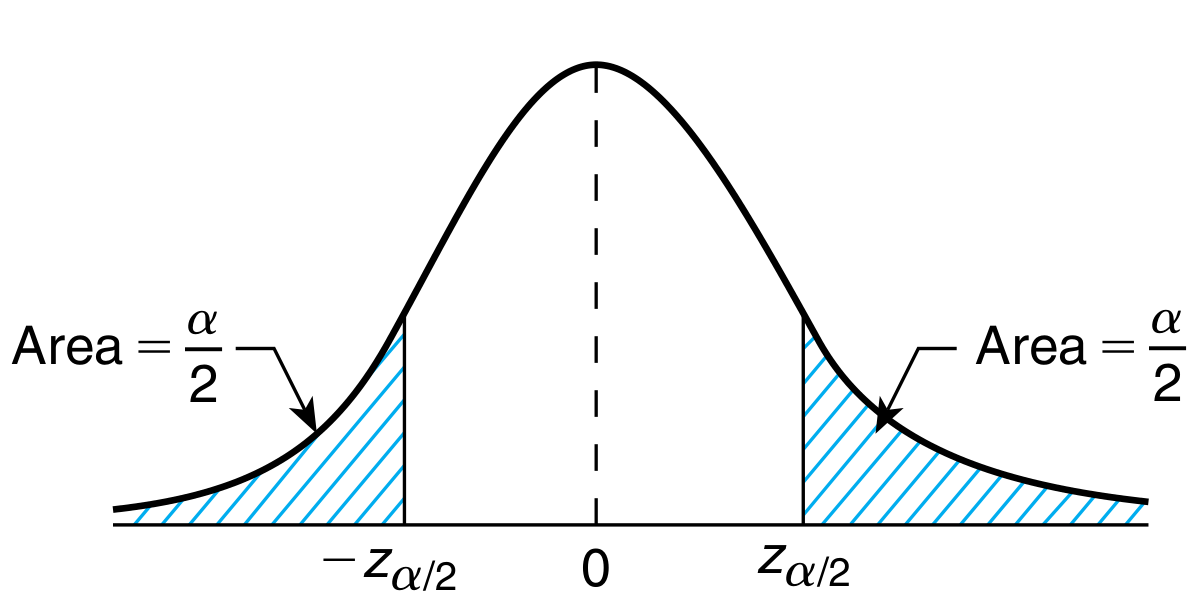
\includegraphics[scale=0.4]{../images/conf_1}
    \centering
    \caption{Visualization of the double sided confidence interval on standard normal.}
    \label{fig:conf_1} %\ref{fig:conf_1}
    \end{figure}

    In a very similar manner, we can calculate the one sided confidence interval. Here, we are only interested in the lower or upper bound of the said interval. The other side is $\inf$ or $-\inf$.
    \begin{align*}
        P(Z > z_{\alpha}) &= \alpha\\
        P(\sqrt{n}\frac{\overline{X} - \mu}{\sigma} > z_{\alpha}) &= \alpha\\
        P(\mu < \overline{x} + z_{\alpha}\frac{\sigma}{\sqrt{n}}) &= \alpha\\
        \Aboxed{\text{Lower $1-\alpha$ confidence interval} &= (-\inf, \overline{x} + z_{\alpha}\frac{\sigma}{\sqrt{n}})}\\
        \\
        P(Z < -z_{\alpha}) &= \alpha\\
        P(\sqrt{n}\frac{\overline{X} - \mu}{\sigma} < -z_{\alpha}) &= \alpha\\
        P(\overline{x} - z_{\alpha}\frac{\sigma}{\sqrt{n}} < \mu) &= \alpha\\
        \Aboxed{\text{Upper $1-\alpha$ confidence interval} &= (\overline{x} - z_{\alpha}\frac{\sigma}{\sqrt{n}}, \inf)}
    \end{align*}

    The interpretation of the right sided confidence interval is that we are $1-\alpha$ confident that the value of the mean is more than the lower end of the interval. In a similar way, the left side interval gives the upper bound on the value of mean with the desired confidence.


    %%%%%%%%%%%%%%%%%%%%%%%%%%%%%%%%%%%%%%%%%%%%%%%%%%%%%%%%%%%%%%%%%%%%%%%%%%%
    \subsubsection{Confidence interval for Mean of Normal Distribution when Variance is Unknown}
    The derivation of confidence intervals in this case is similar to the above, with the only difference of using a t-distribution. Recall
    \begin{align*}
        \sqrt{n} \frac{\overline{X} - \mu}{S} \sim t_{n-1}
    \end{align*}
    where $S$ is the sample variance. Following similar derivation to the known variance case,
    \begin{align*}
        \text{two sided $1 - \alpha$ confidence interval} &= (\overline{x}-t_{\alpha /2, n-1}\frac{s}{\sqrt{n}}, \overline{x}+t_{\alpha /2, n-1}\frac{s}{\sqrt{n}})\\
        \text{Lower $1-\alpha$ confidence interval} &= (-\inf, \overline{x} + t_{\alpha, n-1}\frac{s}{\sqrt{n}})\\
        \text{Upper $1-\alpha$ confidence interval} &= (\overline{x} - t_{\alpha, n-1}\frac{s}{\sqrt{n}}, \inf)
    \end{align*}
    where $s$ is the observed value of the sample variance $S$. However, notice that the intervals calculated will usually be larger than those when the variance is known because t-distribution is heavier tailed than a standard normal and thus has higher variance.

    \begin{figure}[h]
    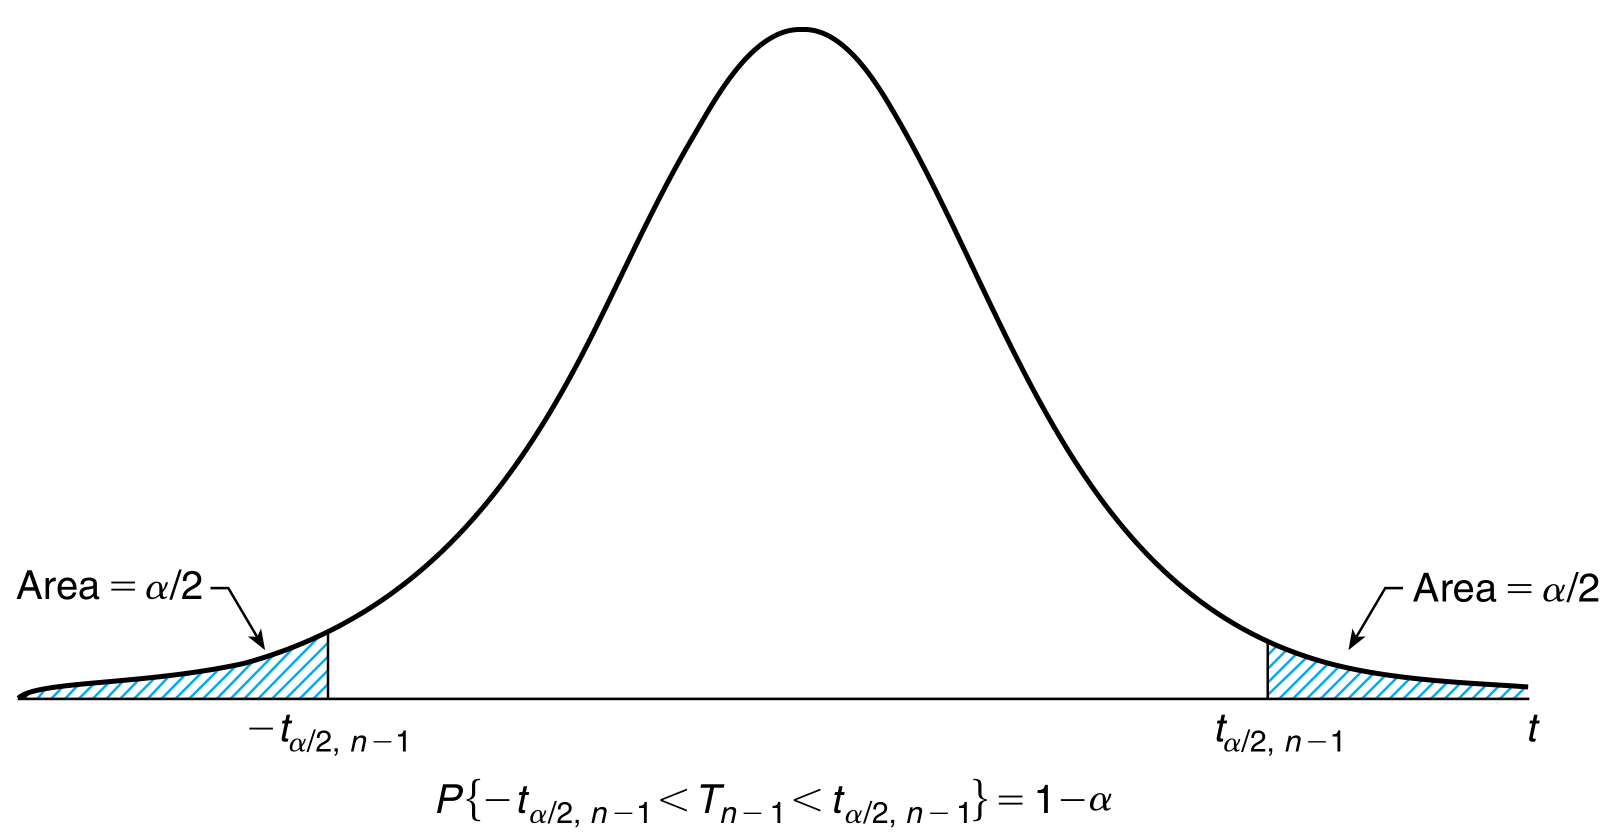
\includegraphics[scale=0.3]{../images/conf_2}
    \centering
    \caption{Visualization of the double sided confidence interval on standard normal.}
    \label{fig:conf_2} %\ref{fig:conf_2}
    \end{figure}

    
    %%%%%%%%%%%%%%%%%%%%%%%%%%%%%%%%%%%%%%%%%%%%%%%%%%%%%%%%%%%%%%%%%%%%%%%%%%%
    \subsubsection{Confidence interval for Variance of Normal Distribution when Mean is Unknown}
    Recall that
    \begin{align*}
        (n-1)\frac{S^{2}}{\sigma^{2}} \sim \chi_{n-1}^{2}
    \end{align*}
    By noting that $\sigma^{2}$ is always positive, we have the following
    \begin{align*}
        \text{two sided $1 - \alpha$ confidence interval} &= (\frac{(n-1)s^{2}}{\chi_{\alpha/2, n-1}^{2}}, \frac{(n-1)s^{2}}{\chi_{1 - \alpha/2, n-1}^{2}})\\
        \text{Lower $1-\alpha$ confidence interval} &= (0, \frac{(n-1)s^{2}}{\chi_{1 - \alpha, n-1}^{2}})\\
        \text{Upper $1-\alpha$ confidence interval} &= (\frac{(n-1)s^{2}}{\chi_{\alpha, n-1}^{2}}, \inf)        
    \end{align*}


    %%%%%%%%%%%%%%%%%%%%%%%%%%%%%%%%%%%%%%%%%%%%%%%%%%%%%%%%%%%%%%%%%%%%%%%%%%%
    \subsubsection{Estimating Difference in Means of Two Normal Populations}
    Suppose the following two independent sets of random variables
    \begin{align*}
        X_{1}, X_{2}, \ldots, X_{n} &\sim \mathcal{N}(\mu_{1}, \sigma_{1}^{2})\\
        Y_{1}, Y_{2}, \ldots, Y_{m} &\sim \mathcal{N}(\mu_{1}, \sigma_{1}^{2})
    \end{align*}

    Then, we are interseted in the distribution of $\mu_{1} - \mu_{2}$. It is intuitive to see that the MLE estimator of this quantity is nothing but $\overline{X} - \overline{Y}$. Also, since $\overline{X}$ and $\overline{Y}$ are both normally distributed,
    \begin{align*}
        \overline{X} - \overline{Y} \sim \mathcal{N}(\mu_{1} - \mu_{2}, \frac{\sigma_{1}^{2}}{n} + \frac{\sigma_{2}^{2}}{m})
    \end{align*}

    Consequently, using the confidence intervals derived for the case of a mean of a single normal distribution, we have the following intervals when the standard deviations are known
    \begin{align*}
        \text{two sided $1 - \alpha$ confidence interval} &= (\overline{x} - \overline{y}-z_{\alpha /2}\sqrt{\frac{\sigma_{1}^{2}}{n} + \frac{\sigma_{2}^{2}}{m}}, \overline{x} - \overline{y}+z_{\alpha /2}\sqrt{\frac{\sigma_{1}^{2}}{n} + \frac{\sigma_{2}^{2}}{m}})\\
        \text{Lower $1-\alpha$ confidence interval} &= (-\inf, \overline{x} - \overline{y}+z_{\alpha /2}\sqrt{\frac{\sigma_{1}^{2}}{n} + \frac{\sigma_{2}^{2}}{m}})\\
        \text{Upper $1-\alpha$ confidence interval} &= (\overline{x} - \overline{y}-z_{\alpha /2}\sqrt{\frac{\sigma_{1}^{2}}{n} + \frac{\sigma_{2}^{2}}{m}}, \inf)
    \end{align*}
    where $\overline{x}$ and $\overline{y}$ are estimates of $\overline{X}$ and $\overline{Y}$ respectively.

    A more challenging scenario arises when the variances are not known. In that case, it is only logical to try to estimate the intervals using sample variances (themselves random variables)
    \begin{align*}
        S_{1}^{2} &= \frac{\sum_{i=1}^{n} (X_{i} - \overline{X})^{2}}{n-1}\\
        S_{2}^{2} &= \frac{\sum_{i=1}^{m} (Y_{i} - \overline{Y})^{2}}{m-1}
    \end{align*}

    However, the distribution useful for deriving the confidence intervals
    \begin{align*}
        \frac{\overline{X} - \overline{Y} - (\mu_{1} - \mu_{2})}{\sqrt{\frac{S_{1}^{2}}{n} + \frac{S_{2}^{2}}{m}}}
    \end{align*}
    is complicated and depends on the unknown variances. The variable is friendly if we assume that the two unknown variances are both same.\newline

    Assuming $\sigma_{1} = \sigma_{2} = \sigma$, it follows
    \begin{align*}
        (n-1)\frac{S_{1}^{2}}{\sigma^{2}} &\sim \chi_{n-1}^{2}\\
        (m-1)\frac{S_{2}^{2}}{\sigma^{2}} &\sim \chi_{m-1}^{2}\\
        (n-1)\frac{S_{1}^{2}}{\sigma^{2}} + (m-1)\frac{S_{2}^{2}}{\sigma^{2}} &\sim \mathcal{\chi_{n+m-2}^{2}}\\
    \end{align*}
    since $S_{1}^{2}$ and $S_{2}^{2}$ are independent chi-square random variables and from section \ref{chi_square} that the sum of such variables is also chi-square.\newline
    We already know
    \begin{align*}
        \frac{\overline{X} - \overline{Y} - (\mu_{1} - \mu_{2})}{\sqrt{\frac{\sigma^{2}}{n} + \frac{\sigma^{2}}{m}}} \sim \mathcal{N}(0, 1)
    \end{align*}
    and we also know that the ratio of a standard normal and the square root of a chi-square divided by it's degrees of freedom is a t-distribution
    \begin{align*}
        \frac{\overline{X} - \overline{Y} - (\mu_{1} - \mu_{2})}{\sqrt{\frac{\sigma^{2}}{n} + \frac{\sigma^{2}}{m}}} \div \sqrt{\frac{(n-1)\frac{S_{1}^{2}}{\sigma^{2}} + (m-1)\frac{S_{2}^{2}}{\sigma^{2}}}{n+m-2}} &\sim t_{n+m-2}
    \end{align*}
    Let
    \begin{align*}
        S_{p} &= \frac{(n-1)S_{1}^{2} + (m-1)S_{2}^{2}}{n + m - 2}
    \end{align*}
    Then,
    \begin{align*}
        P(-t_{\alpha/2, n+m-2} \leq \frac{\overline{X} - \overline{Y} - (\mu_{1} - \mu_{2})}{S_{p}\sqrt{\frac{1}{n} + \frac{1}{m}}} \leq t_{\alpha/2, n+m-2}) &= 1 - \alpha
    \end{align*}
    \begin{align*}
        \text{Two sided $1 - \alpha$ confidence interval} &= (\overline{x} - \overline{y}-t_{\alpha /2, n+m-2}s_{p}\sqrt{\frac{1}{n} + \frac{1}{m}}, \overline{x} - \overline{y}+t_{\alpha /2, n+m-2}s_{p}\sqrt{\frac{1}{n} + \frac{1}{m}})
    \end{align*}
    where $s_{p}$ is the sample estimate for $S_{p}$. Lower confidence interval is derived in a similar fashion to the previous derivations, but the upper confidence interval is the lower confidence interval of $\mu_{2} - \mu_{1}$.

    %%%%%%%%%%%%%%%%%%%%%%%%%%%%%%%%%%%%%%%%%%%%%%%%%%%%%%%%%%%%%%%%%%%%%%%%%%%
    \subsubsection{Confidence Interval for Mean of Bernoulli Random Variable}
    Suppose we obtain a sample of $n$ independent Bernoulli random variables, where the probability of success is $p$. Let $X$ denote the no of successes. Using the CLT for large $n$,
    \begin{align*}
        \frac{X - np}{\sqrt{np(1-p)}} \sim \mathcal{N}(0, 1)
    \end{align*}
    It is not tractable to calculate the confidence intervals from this formulation. Let $\hat{p} = X/n$ denote the MLE of the mean $p$. Substituiting in the denominator of above,
    \begin{align*}
        P(-z_{\alpha/2} \leq \frac{X - np}{\sqrt{n\hat{p}(1-\hat{p})}} \leq z_{\alpha/2}) &\approx 1-\alpha\\
        \text{Two sided $1-\alpha$ confidence interval} &\approx (\hat{p} - z_{\alpha/2}\sqrt{\frac{\hat{p}(1-\hat{p})}{n}}, \hat{p} + z_{\alpha/2}\sqrt{\frac{\hat{p}(1-\hat{p})}{n}})
    \end{align*}
    and one sided confidence intervals can be obtained in similar manner to previous derivations.

    

    %%%%%%%%%%%%%%%%%%%%%%%%%%%%%%%%%%%%%%%%%%%%%%%%%%%%%%%%%%%%%%%%%%%%%%%%%%%
    \subsection{Evaluating an Estimator}
    Let $\boldsymbol{X} = (X_{1}, X_{2}, \ldots, X_{n})$ be the set of random variables sampled from a population whose parameters are defined by $\theta$. Let $d(\boldsymbol{X})$ denote an estimator of $\theta$. Then
    \begin{align*}
        r(d, \theta) = E[(d(\boldsymbol{X}) - \theta)^{2}]
    \end{align*}
    denotes the mean squared estimator of $\boldsymbol{X}$. Although it is rare to find an estimator that minimizes this error, we can certainly find the minima under the set of estimators satisfying a certain criteria.\newline
    The bias of an estimator is defined as
    \begin{align*}
        b_{\theta}(d) = E[d(\boldsymbol{X})] - \theta
    \end{align*}
    If the bias is zero, then the estimator is called an \textbf{unbiased estimator}. That is, the expected value of the estimator is same as the parameter being estimated.\newline

    For an unbiased estimator, the mean square error is
    \begin{align*}
        r(d, \theta) &= E[(d(\boldsymbol{X}) - \theta)^{2}]\\
        &= E[(d(\boldsymbol{X}) - E[d(\boldsymbol{X})])^{2}]\\
        &= Var(d(\boldsymbol{X}))
    \end{align*}
    i.e., the mean squared error of an unbiased estimator is equal to its variance.\newline

    Let $X_{1}, X_{2}, \ldots, X_{n}$ be sampled from a distribution whose mean is $\theta$. Then,
    \begin{align*}
        d(\boldsymbol{X}) &= \sum_{i=1}^{n} \lambda_{i} X_{i}\\
        \text{and \:} \sum_{i=1}^{n}\lambda_{i} &= 1
    \end{align*}
    is also an unbiased estimator because
    \begin{align*}
        E[\sum_{i=1}^{n} \lambda_{i} X_{i}] &= \sum_{i=1}^{n} \lambda_{i} E[X_{i}]\\
        &= \theta \sum_{i=1}^{n}\lambda_{i}\\
        &= \theta
    \end{align*}

    
    %%%%%%%%%%%%%%%%%%%%%%%%%%%%%%%%%%%%%%%%%%%%%%%%%%%%%%%%%%%%%%%%%%%%%%%%%%%
    \subsubsection{Combining Unbiased Estimators}
    Suppose we have $n$ unbiased estimators $d_{1}, \ldots, d_{n}$ for a parameter $\theta$ with different independent variances
    \begin{align*}
        E[d_{i}] = \theta \quad Var(d_{i}) = \sigma_{i}^{2}
    \end{align*}
    Then, a weighted combination of these estimators is also an unbiased estimator of $\theta$ (assuming that the weights sum up to 1). Suppose we wish to find a set of weights that minimize the mean squared error to get the best estimator, then
    \begin{gather*}
        d = \sum_{i=1}^{n} w_{i} d_{i} \text{\: where $\sum_{i=1}^{n} w_{i} = 1$}\\
        r(d, \theta) = Var(d) \text{\:(derived above)}\\
        Var(d) = Var(\sum_{i=1}^{n} w_{i} d_{i})\\
        = \sum_{i=1}^{n}w_{i} Var(d_{i}) \text{\: by independence}\\
        = \sum_{i=1}^{n}w_{i} \sigma_{i}^{2}\\
        \text{So we minimize\:} \sum_{i=1}^{n}w_{i} \sigma_{i}^{2} - \lambda(\sum_{i=1}^{n} w_{i}-1)\\
        \text{Taking the derivative for any $i$, \:} 0 = 2\sigma_{i} w_{i} - \lambda\\
        \text{Using \:}\sum_{i=1}^{n} w_{i} = 1\\
        w_{i} = \frac{1/\sigma_{i}^{2}}{1/\sigma_{1}^{2} + 1/\sigma_{2}^{2} + \cdots + 1/\sigma_{n}^{2}}
    \end{gather*}
    or, the weights for the estimators are inversely proportional to their individual variances. This is useful in situations when we have $n$ independent results for evaluation of a parameter, and we want to increase our confidence in the estimator by combining all these independent results.\newline


    %%%%%%%%%%%%%%%%%%%%%%%%%%%%%%%%%%%%%%%%%%%%%%%%%%%%%%%%%%%%%%%%%%%%%%%%%%%
    \subsubsection{Relation between Bias and Variance}
    The result obtained above that the mean squared error of an unbiased estimator is it's variance can be generalized for the case of any estimator as follows
    \begin{align*}
        r(d, \theta) &= E[(d - \theta)^{2}]\\
        &= E[(d - E[d] + E[d] -\theta)^{2}]\\
        &= E[(d - E[d])^{2} + (E[d] - \theta)^{2} + 2(d - E[d])(E[d] - \theta)]\\
        &= E[(d - E[d])^{2}] + E[(E[d] - \theta)^{2}] + 2(E[d] - \theta)E[d - E[d]]\\
        &= E[(d - E[d])^{2}] + (E[d] - \theta)^{2}\\
        \Aboxed{r(d, \theta) &= Var(d) + b_{\theta}^{2}(d)}\\
    \end{align*}
    where we have noted that $E[d - E[d]] = E[d] - E[d] = 0$ and $E[d] - \theta$ is a constant since $E[d]$ itself is a constant.


    %%%%%%%%%%%%%%%%%%%%%%%%%%%%%%%%%%%%%%%%%%%%%%%%%%%%%%%%%%%%%%%%%%%%%%%%%%%
    \subsection{Bayes Estimator}
    The Bayes estimator is the expected value of the parameter given the data. It utilizes the Bayes theorem in order to arrive at the estimator value
    \begin{align*}
        E[\theta|X_{1} = x_{1}, X_{2} = x_{2}, \ldots, X_{n} = x_{n}] &= \int \theta f(\theta|x_{1}, x_{2}, \ldots, x_{n})\\
        f(\theta|x_{1}, x_{2}, \ldots, x_{n}) &= \frac{p(\theta) f(x_{1}, x_{2}, \ldots, x_{n} | \theta)}{\int p(\theta) f(x_{1}, x_{2}, \ldots, x_{n} | \theta) d\theta}
    \end{align*}
    where $p(\theta)$ is the assumed prior distribution on the parameter $\theta$. Based on our knowledge of the process, this can be uniform, normal etc.
\end{document}